\documentclass[conference]{IEEEtran}
\IEEEoverridecommandlockouts

\usepackage{cite}
\usepackage{amsmath,amssymb,amsfonts}
\usepackage{algorithmic}
\usepackage{graphicx}
\usepackage{textcomp}
\usepackage{xcolor}
\usepackage{hyperref}

\begin{document}

\title{StockSense: Multi-Target Trading Automation with Deep Reinforcement Learning}

\author{
  \IEEEauthorblockN{Yan-Fu Chen}
  \IEEEauthorblockA{
    \textit{Dept. of Computer Science} \\
    \textit{National Tsing-Hua University}\\
    Hsinchu, Taiwan \\
    aaaronyanfu@gmail.com
  }
  \and
  \IEEEauthorblockN{Yi-Ning Chang}
  \IEEEauthorblockA{
    \textit{Dept. of Computer Science} \\
    \textit{National Tsing-Hua University}\\
    Hsinchu, Taiwan \\
    changyn@gapp.nthu.edu.tw
  }
  \and
  \IEEEauthorblockN{Sheng-You Chien}
  \IEEEauthorblockA{
    \textit{Dept. of Computer Science} \\
    \textit{National Tsing-Hua University}\\
    Hsinchu, Taiwan \\
    s99086tobby@gmail.com
  }
  \and
  \IEEEauthorblockN{Bo-Yi Mao}
  \IEEEauthorblockA{
    \textit{Dept. of Computer Science} \\
    \textit{National Tsing-Hua University}\\
    Hsinchu, Taiwan \\
    dogeon188@gapp.nthu.edu.tw
  }
  \and
  \IEEEauthorblockN{Jie-Hung Chen}
  \IEEEauthorblockA{
    \textit{Dept. of Computer Science} \\
    \textit{National Tsing-Hua University}\\
    Hsinchu, Taiwan \\
    jiehongchen726@gmail.com
  }
  \and
  \IEEEauthorblockN{Yi-Hsueh Chu}
  \IEEEauthorblockA{
    \textit{Dept. of Computer Science} \\
    \textit{National Tsing-Hua University}\\
    Hsinchu, Taiwan \\
    ethan111062332@gapp.nthu.edu.tw
  }
}

\maketitle

\begin{abstract}

  In this paper, we leverage deep reinforcement learning (DRL) to automate multi-target trading, where the goal is to optimize trading decisions across a portfolio of assets. We propose a flexible and extensible architecture that supports multiple stocks, various trading strategies, and different reinforcement learning algorithms. We evaluate the performance of our models on a real-world dataset and compare them with traditional buy-and-hold strategies.

  Our results show that our DRL models outperform the buy-and-hold strategy in terms of annualized return and cumulative return. However, the DRL models exhibit higher risk, which demonstrates the trade-off between return and risk in multi-target trading.

\end{abstract}

\begin{IEEEkeywords}
  computational finance, deep reinforcement learning, algorithmic trading, multi-target trading
\end{IEEEkeywords}

\section{Introduction}

An automatic, algorithmic way of stock trading, leveraging the swiftness and accuracy of computer systems, has long been a persuit of many. With the rise of machine learning and deep learning, the possibility of using these technologies to predict stock prices and make trading decisions has become a reality.

Many studies have tackled the problem of stock price prediction using machine learning models, such as Support Vector Machines (SVMs), Convolutional Neural Networks (CNNs), and Recurrent Neural Networks (RNNs). These models have shown promising results in forecasting stock prices, capturing temporal dependencies, and extracting relevant features from raw data.

However, few works have made a formal attempt to combine algorithmic trading, deep reinforcement learning, and multi-target trading. In this paper, we aim to address this gap by summarizing and extending the current state-of-the-art algorithms and methodologies for multi-target trading automation using deep reinforcement learning, and comparing their performance on a real-world dataset.

\section{Related Works}

Even though the Efficient Market Hypothesis (EMH) posits that stock prices reflect all available information, and thus cannot be predicted consistently, many studies have shown that stock prices exhibit predictable patterns and can be forecasted to some extent. Various approaches have been proposed, differing in learning algorithms and objectives. In recent years, deep reinforcement learning (DRL) has gained significant attention due to its ability to learn complex trading strategies directly from market data.

\subsection{Stock Price Prediction}

Most studies have focused on predicting stock prices using various machine learning models. Traditional statistical methods such as ARIMA and GARCH have been widely used for time series forecasting. However, financial time series are often non-stationary and exhibit volatility changes, making it challenging to capture their underlying patterns with smoothened models.

With the advent of machine learning and deep learning, more sophisticated models have been developed. Convolutional Neural Networks (CNNs) and Recurrent Neural Networks (RNNs), including Long Short-Term Memory (LSTM) networks, have shown promising results in stock price prediction. These models can automatically extract relevant features from raw data and capture temporal dependencies, making them well-suited for financial time series analysis.

Support Vector Machines (SVMs) have been applied to stock predictions in many works. Phayung et al. \cite{phayung2013} applied Support Vector Regression (SVR) and combines different windowing functions to predict stock prices. Their model showed good performance in predicting short-term stock prices. Similarly, Tripathy \cite{tripathy2019} demonstrated that SVMs are effective in highly volatile markets, and it performs better in short-term and medium-term predictions compared to long-term predictions. Also, Zhang et al. \cite{zhang2017} proposed a periodic updating SVM model that can adapt to changing market conditions, which showed competitive performance compared to the random walk model proposed by the EMH.

Zhang et al. \cite{zhang2017} proposed a State Frequency Memory (SFM) recurrent neural network to capture the multi-frequency trading patterns in stock prices. They demonstrated that their model showed competitive performance compared to traditional methods. Fischer and Krauss \cite{fischer2018} applied LSTM networks to rank stocks based on their future returns and showed that their model could outperform traditional ranking methods.

More advanced models have also been applied to stock price prediction in recent years. Feng et al. \cite{feng2019an} proposed an adversarial learning framework that outperformed SOTA methods in terms of prediction accuracy. Koa et al. \cite{koa2023} developed a combination of Variational Autoencoders (VAEs) and diffusion models to capture the latent structure of financial time series. Gao et al. \cite{gao2023} proposed a transformer-based model that outperformed traditional methods in terms of portfolio returns and Sharpe ratios.

\subsection{Algorithmic Trading}

Deep reinforcement learning (DRL), a branch of machine learning where an agent learns to make decisions by interacting with an environment to maximize cumulative rewards, is capable of learning complex trading strategies directly from market data, making it an attractive approach for algorithmic trading. For example, Deep Q-Learning (DQN) has been widely applied to stock trading for decision-making in dynamic and uncertain environments. Jiang et al. \cite{jiang2017} developed a deep reinforcement learning model that can adapt to changing market conditions and showed competitive performance compared to traditional methods. Liu et al. \cite{liu2022finrl} proposed a deep reinforcement learning library, FinRL, tailored for financial markets, enabling multi-stock trading strategies. Their library provides a comprehensive set of tools for developing and evaluating trading strategies using reinforcement learning, including various environments, algorithms, and evaluation metrics.

Despite these advancements in stock price prediction, they are usually evaluated on historical data and do not consider the trading strategy's performance in real-world scenarios. few works have addressed the challenges of multi-target trading, where the goal is to optimize trading decisions across a portfolio of assets. Multi-target trading involves managing multiple stocks simultaneously, considering their interdependencies and correlations to maximize overall portfolio returns.

One notable work in this area is by Feng et al. \cite{feng2019rank}, who proposed an improved ranking model that can generate trading signals based on the predicted stock returns. Importantly, they considered the relationship between different stocks that conveys valuable information for trading decisions.

\section{Methodology}

The utilized multi-target trading architecture is designed to handle multiple stock assets simultaneously, optimizing trading decisions across a portfolio rather than focusing on a single stock. To address this challenge, we leverage DRL algorithms with a flexible environment that supports multi-asset trading. Below, we outline the key components of the architecture:

\subsection{Reinforcement Learning Overview}

Reinforcement learning is based on the interaction between an \textbf{agent} and an \textbf{environment}. The agent observes the state of the environment, takes actions, and receives rewards based on the results of those actions. The goal of the agent is to learn an optimal policy that maximizes the cumulative reward over time.

\begin{itemize}
  \item \textbf{State ($S_t$)}: Represents the information observed by the agent from the environment at time $t$.
  \item \textbf{Action ($A_t$)}: The decision made by the agent at time $t$, such as buying, selling, or holding stocks.
  \item \textbf{Reward ($R_t$)}: A scalar feedback signal that evaluates the action taken by the agent in a specific state.
  \item \textbf{Policy ($\pi$)}: A mapping from states to actions, guiding the agent's decision-making process.
  \item \textbf{Q-Function ($Q(s, a)$)}: Represents the expected cumulative reward of taking action $a$ in state $s$ and following the policy thereafter.
\end{itemize}

We use advanced RL algorithms such as \textit{Deep Q-Network (DQN)}, \textit{Advantage Actor-Critic (A2C)}, and \textit{Proximal Policy Optimization (PPO)} to train our agents.

\subsection{Environment}

The environment simulates a stock market, incorporating realistic features such as price changes, transaction costs, and investment constraints. It provides the agent with state information derived from historical market data, enabling the agent to learn and make trading decisions.

\begin{itemize}
  \item \textbf{Data Source}: The environment accepts a list of Pandas DataFrames containing historical stock price data for multiple assets. For each DataFrame, the columns represent the OHLCV data (open, high, low, close prices, and trading volume) at each time step.
  \item \textbf{Implementation}: The environment is implemented by extending the Gymnasium \texttt{Env} class, allowing seamless integration with reinforcement learning frameworks.
\end{itemize}

\subsection{State Representation}

The state representation is critical for effective learning. Since raw stock market data varies greatly in scale and lacks direct interpretability, we preprocess and normalize it into meaningful features:

\begin{itemize}
  \item \textbf{Normalized Price Features}:
    \begin{align*}
      \text{Open\%} &= \frac{\text{Open}}{\text{Close}}, \quad \text{High\%} = \frac{\text{High}}{\text{Close}}, \quad \text{Low\%} = \frac{\text{Low}}{\text{Close}}
    \end{align*}
  \item \textbf{Percentage Change of Close}: Measures the relative change in the close price compared to the previous day.
  \item \textbf{Normalized Volume}: Volume as a percentage of the maximum trading volume within a specified time window (100 days).
\end{itemize}

The agent observes the last five days of these features, creating a sliding window of information to capture short-term trends.

\subsection{Actions}

The action space defines how the agent interacts with the environment. In our implementation, we support two modes of trading actions:

\begin{enumerate}
  \item \textbf{All-In Mode}: The agent selects a single stock to allocate 100\% of its capital.
  \item \textbf{Proportional Allocation Mode}: The agent determines the percentage of capital to allocate across multiple stocks, enabling diversified strategies.
\end{enumerate}

This flexibility allows the agent to explore both high-risk and balanced investment strategies.

\subsection{Reward Function}

We use the \textbf{logarithmic gain ratio} as the reward function to evaluate the performance of the agent's decisions. This reward structure emphasizes proportional gains, penalizes losses, and encourages consistent growth. The reward for a given action is calculated as:
\begin{align*}
  R_t = \log\left(\frac{\text{Portfolio Value}_{t}}{\text{Portfolio Value}_{t-1}}\right)
\end{align*}

This formulation accounts for transaction costs and ensures that the agent focuses on maximizing net returns.

\subsection{Agent Design}

To solve the trading problem effectively, we utilize three reinforcement learning algorithms:

\begin{itemize}
  \item \textbf{Deep Q-Network (DQN)}: Uses a neural network to approximate the Q-function. It is particularly effective for discrete action spaces and leverages experience replay and target networks for stability.
  \item \textbf{Advantage Actor-Critic (A2C)}: A policy-gradient method that combines value-based and policy-based approaches. It learns both a value function (critic) and a policy (actor) simultaneously, enabling efficient exploration.
  \item \textbf{Proximal Policy Optimization (PPO)}: A robust and scalable policy-gradient method. It improves training stability by constraining policy updates to avoid drastic changes, ensuring better convergence.
\end{itemize}

Each algorithm is trained to optimize portfolio returns while managing risks and transaction costs.

\section{Experiments}

\subsection{Dataset}

We obtained the stock price data from Yahoo! Finance \cite{yahoofinance} using the yfinance Python library \cite{yfinance}, and preprocess the data to fit the requirements of our trading environment. The dataset used in our experiments includes the daily OHLCV data for the following stocks: Microsoft (MSFT), Apple (AAPL), American Express (AXP), Amgen (AMGN), Cisco Systems (CSCO), Honeywell (HON), IBM (IBM), and Coca-Cola (KO). It contains data points spanning from January 1, 2000 to December 1, 2024.

The dataset is split into three parts:
\begin{itemize}
  \item Training Data: First 70\% of the data (from January 1, 2000 to June 12, 2017).
  \item Validation Data: Next 10\% of the data (from June 13, 2017 to December 6, 2019).
  \item Testing Data: Last 20\% of the data (from December 7, 2019 to December 1, 2024).
\end{itemize}

The training data is used to train the reinforcement learning models, while the validation data is used to tune hyperparameters and prevent overfitting. The testing data is used to evaluate the performance of the trained models.

To visualize the historical stock prices used in our experiments, we plot the closing prices of the selected stocks over the entire dataset period in Figure \ref{fig:price_history}.

\begin{figure}[htbp]
  \centerline{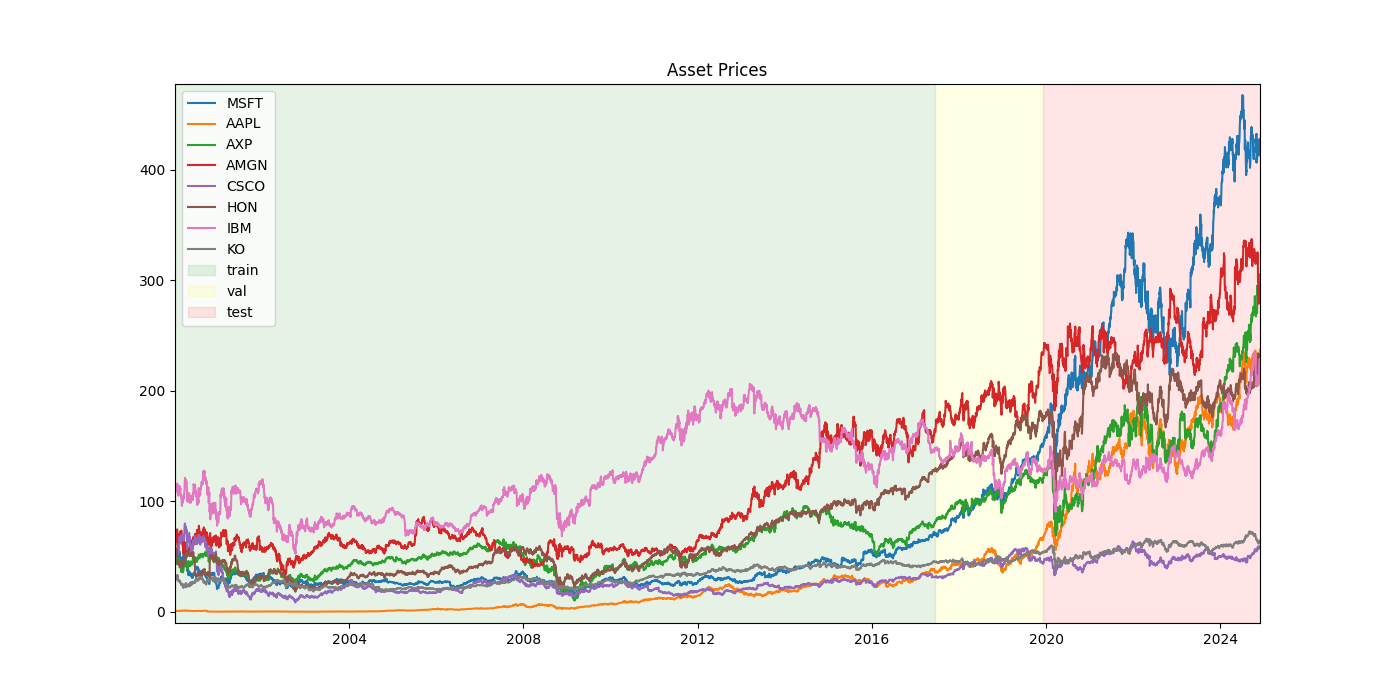
\includegraphics[width=0.5\textwidth]{figs/prices.png}}
  \caption{Historical closing prices of selected stocks from January 1, 2000 to December 1, 2024.}
  \label{fig:price_history}
\end{figure}

\subsection{Evaluation Metrics}

% 張 簡
% Introduce the evaluation metrics used
Backtesting is a common method to evaluate the performance of a predictive model in the financial domain. It simulates the trading strategy on historical data to estimate the strategy's performance.

We use FinRL \cite{liu2022finrl}, a powerful deep reinforcement learning library to perform backtest on our trading strategy. Our reinforcement learning model is compared with the buy-and-hold (B\&H) strategy, which buys and holds the stock for the entire trading period, on the DJI Index. DJI Index is a stock market index that measures the stock performance of 30 large companies listed on stock exchanges in the United States.

Our models are evaluated based on the following metrics:
\begin{itemize}
  \item Annualized Return: The annualized return of the trading strategy.
  \item Cumulative Return: The cumulative return of the trading strategy.
  \item Maximum Drawdown: The maximum loss from a peak (highest point) to a trough (lowest point) of a trading strategy. A higher maximum drawdown indicates the trading strategy has higher risk.
  \item Annualized Volatility: The annualized volatility is defined as the standard deviation of the asset's yearly logarithmic return. A higher annualized volatility indicates the trading strategy has higher risk.
  \item Sharpe Ratio: As measure of the risk-adjusted return of the trading strategy, the Sharpe ratio is defined as:
    \begin{equation}
      \text{Sharpe Ratio} = \frac{E[R_p - R_f]}{\sigma_p}
    \end{equation}
    where $R_p$ is the asset return of the trading strategy, $\sigma_p$ is the standard deviation of the asset excess return, and $R_f$ is the risk-free return (such as a U.S. Treasury security). Therefore, The Sharpe ratio characterizes how well the return of an asset compensates the investor for the risk taken. A higher Sharpe ratio indicates the strategy can generate higher returns with lower risk.
  \item Calmar Ratio:
    The Calmar ratio is defined as the ratio of the annualized return to the maximum drawdown of the trading strategy:
    \begin{equation}
      \text{Calmar Ratio} = \frac{\text{Annualized Return}}{\text{Maximum Drawdown}}
    \end{equation}
    A higher Calmar ratio indicates the strategy can generate higher returns with lower downside risk. Compared to the Sharpe ratio, the Calmar ratio focuses on the downside risk of the trading strategy.

  \item Sortino Ratio: Sortino ratio is a variation of the Sharpe ratio that only considers the downside risk of the trading strategy. It is defined as:
    \begin{equation}
      \text{Sortino Ratio} = \frac{E[R_p - R_f]}{\sigma_d}
    \end{equation}
    where $\sigma_d$ is the standard deviation of the asset downside return. A higher Sortino ratio indicates the strategy can generate higher returns with lower downside risk.
  \item Omega Ratio: The Omega ratio is a risk-return measure that evaluates the probability of achieving a certain return. It is defined as:
    \begin{equation}
      \text{Omega Ratio} = \frac{P(R_p > R_f)}{P(R_p < R_f)}
    \end{equation}
    where $P(R_p > R_f)$ is the probability of achieving a return greater than the risk-free rate, and $P(R_p < R_f)$ is the probability of achieving a return less than the risk-free rate. A higher Omega ratio indicates the strategy has a higher probability of achieving a return greater than the risk-free rate.
\end{itemize}

\subsection{Results}
This section presents the experimental results of applying different models and strategies to stock market prediction and portfolio management. The model we implemented in this study is the Deep Q-Network (DQN), and it is compared against several baseline strategies.

\subsubsection{Asset Prices Over Time}
Figure \ref{fig:price_history} shows the historical performance of selected stocks, including MSFT, AAPL, AXP, AMGN, CSCO, HON, IBM, and KO. The plot is segmented into three periods: the training period (green background), the validation period (yellow background), and the test period (pink background).

From the chart, it is evident that AAPL and MSFT exhibit the most significant growth trajectories, particularly during the test period, where their values rise steeply. MSFT surpasses all other stocks in terms of cumulative performance, highlighting its dominance in the observed timeframe. This exceptional growth could be attributed to factors such as market innovation, strong earnings, or favorable macroeconomic conditions. Conversely, stocks like KO and IBM display relatively flat trajectories, indicating limited growth potential or consistent performance without major volatility.

AMGN demonstrates a notable rise during the validation period but appears to plateau in the test period, which could reflect sector-specific trends or external market influences that hindered its continued growth. AXP, on the other hand, shows moderate growth but remains significantly behind the tech-driven advancements of AAPL and MSFT, underscoring the variability in performance across different industries.

\subsubsection{Model Performance Comparison}

Table \ref{tab:results} and Figure \ref{fig:returns} present the performance comparison of the B\&H baseline against DRL strategies, including DQN, A2C, and PPO. The evaluation metrics include annualized return, cumulative return, maximum drawdown, Sharpe ratio, Calmar ratio, annualized volatility, and Sortino ratio.

\begin{itemize}
  \item \textbf{Cumulative Returns:} The DQN model achieves the highest cumulative returns among all strategies, significantly outperforming traditional approaches like B\&H. This demonstrates the DQN's capability to dynamically adjust portfolio allocations and capitalize on market inefficiencies.
  \item \textbf{Sharpe Ratio:} The Sharpe ratio for DQN is notably higher than that of most baseline strategies, indicating superior risk-adjusted returns. This metric highlights the model's ability to balance returns against market volatility effectively.
  \item \textbf{Maximum Drawdown:} Despite its strengths, the DQN model exhibits a relatively large maximum drawdown. This underscores its susceptibility to sharp market downturns, potentially due to overfitting or high sensitivity to volatile conditions.
  \item \textbf{Strategy Observations:} For the tested strategies, the following observations are made:
    \begin{itemize}
      \item \textbf{B\&H:} This strategy delivers stable returns with a relatively higher Sharpe ratio compared to other baseline models. While it minimizes risk and avoids major drawdowns, its lack of adaptability prevents it from taking full advantage of upward market trends, resulting in moderate cumulative returns.
      \item \textbf{DQN:} DQN achieves the highest cumulative returns and Sharpe ratio among all strategies, indicating its superior performance in optimizing portfolio allocations and managing risk. However, its larger maximum drawdown suggests potential vulnerabilities to sudden market downturns or overfitting to specific market conditions.
      \item \textbf{A2C:} A2C achieves moderate performance with higher cumulative returns than PPO but struggles to match the adaptability of more sophisticated models. Its Sharpe ratio indicates balanced risk-adjusted returns, though it remains lower than that of DQN.
      \item \textbf{PPO:} Although PPO demonstrates some capability in managing risk, its cumulative returns and Sharpe ratio are the lowest among the three. This suggests that PPO failed to effectively capture upward market trends during the test period and did not outperform the other baseline strategies in balancing risk and reward
    \end{itemize}

\end{itemize}

\section{Discussion}
This section analyzes the experimental results and provides potential insights and improvements for the DQN model based on its performance.

\subsection{Analysis of Results}
\begin{itemize}
  \item \textbf{DQN's Strengths:} The exceptional cumulative returns achieved by the DQN model stem from its use of deep Q-learning, which enables it to efficiently learn optimal policies for asset allocation by mapping states to value estimates. This adaptability enables the model to exploit trends in high-performing assets, such as AAPL and MSFT, particularly during periods of rapid growth. Furthermore, the consistently high Sharpe ratio demonstrates the model's capacity to manage risk effectively while maximizing returns.
  \item \textbf{Drawdown Challenges:} Despite its strong performance metrics, the DQN model's larger maximum drawdown compared to baseline strategies suggests a potential vulnerability to sudden market downturns. This may arise from overfitting to specific market conditions during training or an over-reliance on short-term signals that increase risk exposure.
\end{itemize}

\subsection{Potential Improvements}
\begin{itemize}
  \item \textbf{Regularization and Robustness:} To address overfitting, implementing regularization techniques, such as dropout layers or weight decay, could improve the model's generalization capabilities. Additionally, ensemble methods could provide more stable performance across different market conditions by reducing the impact of outliers.
  \item \textbf{Risk Management:} Incorporating explicit risk management objectives, such as drawdown constraints or volatility penalties, into the reward function could help mitigate excessive risk exposure. By aligning the model's behavior with practical investment strategies, these enhancements could improve its robustness in real-world applications.
  \item \textbf{Feature Engineering:} Expanding the feature set with macroeconomic indicators, such as interest rates or inflation data, and alternative data sources, such as sentiment analysis from news or social media, could improve the model's predictive capabilities. Additionally, incorporating sector-specific indicators may help capture trends that are unique to particular industries.
  \item \textbf{Dynamic Reward Functions:} Modifying the reward function to account for long-term performance metrics, such as capital preservation or reduced portfolio turnover, could encourage more sustainable and consistent investment strategies. This would also address concerns regarding high transaction costs associated with frequent portfolio rebalancing.
\end{itemize}

In conclusion, while the DQN model demonstrates significant potential in outperforming traditional portfolio management strategies, careful consideration of its limitations, particularly regarding risk and robustness, is crucial for practical deployment. Future research could explore the integration of multi-agent reinforcement learning frameworks or hybrid approaches to enhance the model's adaptability and performance in complex and dynamic financial markets.

\begin{table}[htbp]
  \centering
  \caption{Performance comparison of the strategies on our dataset.}
  \begin{tabular}{|c|c|c|c|c|}
    \hline
    \textbf{Evaluation} & \multicolumn{4}{|c|}{\textbf{Model}} \\
    \cline{2-5}
    \textbf{Metric} & \textit{\textbf{DQN}} & \textit{\textbf{A2C}} & \textit{\textbf{PPO}} & \textit{\textbf{Buy-and-Hold}} \\
    \hline
    Annualized Return & \underline{0.3122} & 0.2119 & 0.0192 & 0.2387 \\
    \hline
    Cumulative Return & \underline{0.3969} & 0.2667 & 0.0237 & 0.3001 \\
    \hline
    Maximum Drawdown & -0.1807 & -0.1549 & -0.2074 & \underline{-0.0678} \\
    \hline
    Sharpe Ratio & 1.4614 & 1.0595 & 0.1955 & \underline{2.1126} \\
    \hline
    Calmar Ratio & 1.7389 & 1.3682 & 0.0925 & \underline{3.5230} \\
    \hline
    Annualized Volatility & 0.1999 & 0.2012 & 0.1941 & \underline{0.1043} \\
    \hline
    Sortino Ratio & 1.5270 & 1.4550 & 0.2661 & \underline{3.2108} \\
    \hline
  \end{tabular}
  \begin{tabular}{p{0.45\textwidth}}
    \textit{Note:} The best performance for each metric is underlined.
  \end{tabular}
  \label{tab:results}
\end{table}

\begin{figure}[htbp]
  \centerline{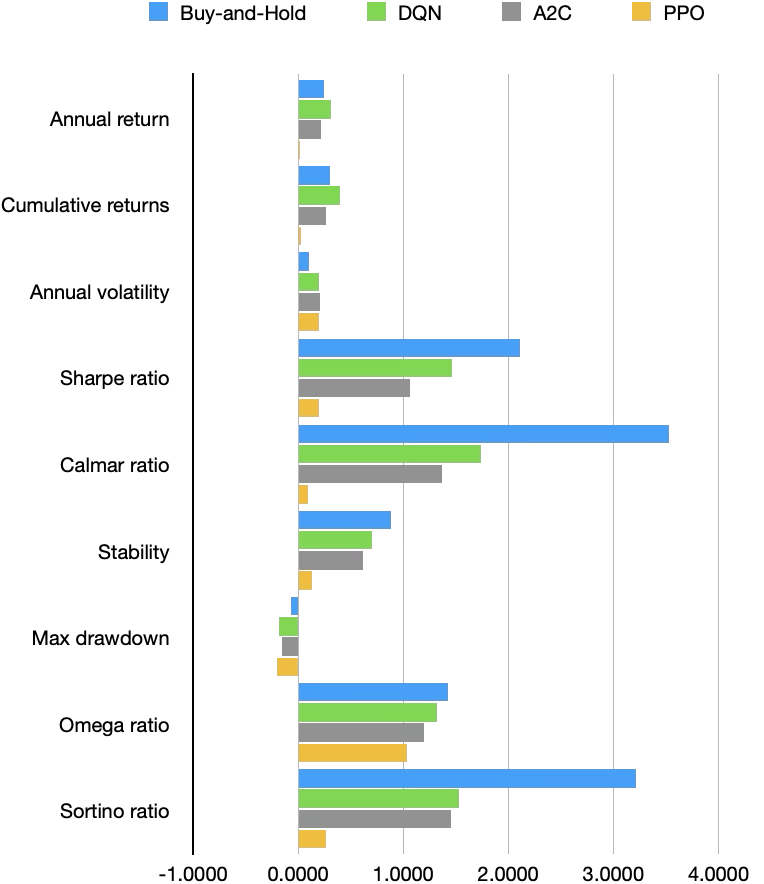
\includegraphics[width=0.4\textwidth]{figs/results.png}}
  \caption{Performance comparison of the strategies on our dataset.}
  \label{fig:returns}
\end{figure}

\section{Conclusion}

In this paper, we proposed a flexible and extensible architecture for multi-target trading automation using deep reinforcement learning. We evaluated several reinforcement learning algorithms, including DQN, A2C, and PPO, on a real-world dataset containing historical stock price data for multiple assets.

Our results show that our DRL models outperform the baseline buy-and-hold strategy in terms of annualized return and cumulative return. However, the DRL models exhibit higher risk, as indicated by the maximum drawdown and annualized volatility. As our model is optimized for return, such risky behavior is expected. This demonstrates the trade-off between return and risk in multi-target trading.

The forementioned results also suggest that our models may benefit from additional risk management techniques to reduce downside risk and improve overall performance. With a more sophisticated reward function that considers risk-adjusted returns, we can potentially achieve a better balance between return and risk. Furthermore, incorporating additional features such as technical indicators, market sentiment, and macroeconomic factors could enhance the model's predictive power and robustness. Future work could explore these directions to further improve the performance of our models.

\section{Data and Code Availability}

Stock price data used in this study is publicly available from Yahoo! Finance \cite{yahoofinance}, and is obtained using the yfinance Python library \cite{yfinance}. Cryptocurrency price data is obtained from the Binance API \cite{binanceapi} using the ccxt Python library \cite{ccxt}.

All code for data fetching, data preprocessing, model training, and evaluation is available at \url{https://github.com/Dogeon188/StockSense}. Any updates or changes to the code will be reflected in the GitHub repository.

\section{Author Contribution Statements}

\begin{itemize}
  \item \textbf{Y. Chen} \textit{(16.9\%)}: study research, methodology design.
  \item \textbf{Y. Chang} \textit{(16.7\%)}: result analysis, proposal presentation, evaluation metrics.
  \item \textbf{B. Mao} \textit{(16.7\%)}: data curation, video presentation, project outline.
  \item \textbf{S. Chien} \textit{(16.5\%)}: methodology design, result analysis.
  \item \textbf{J. Chen} \textit{(16.5\%)}: methodology design, evaluation metrics.
  \item \textbf{Y. Chu} \textit{(16.5\%)}: study research, data curation.
\end{itemize}

\bibliographystyle{IEEEtran}
\bibliography{refs}

\end{document}